\documentclass{article}
\usepackage[preprint,nonatbib]{neurips_2025}
\usepackage[T1]{fontenc}
\usepackage[utf8]{inputenc}
\usepackage{amsmath,amssymb,booktabs,graphicx,caption,url,hyperref}
\hypersetup{colorlinks=true,linkcolor=blue,citecolor=blue,urlcolor=blue}
\title{Daily Temperature Forecasting\\with Seasonal Regression and ARMA Errors}
\author{Jiayu \qquad Laman\\CPTS 570 Machine Learning, Fall 2026}
\begin{document}
\maketitle
\begin{abstract}
This study examines the predictive contribution of annual seasonality and
short-term residual dependence to daily mean temperature forecasting at
Pullman/Moscow Regional Airport. Using 2,191 NOAA GSOD observations from
2019--2024, seasonal regression with ARMA errors is compared with persistence,
independent-error seasonal regression, and nonseasonal ARIMA. Chronological
validation selects three harmonic pairs with ARMA(1,1) errors. Following
refitting through 2023, a rolling-origin evaluation with fixed parameters in
2024 yields RMSEs of 2.405\,$^\circ$C and 4.019\,$^\circ$C at one- and
seven-day horizons. The seven-day improvement over seasonal regression is
0.015\,$^\circ$C. Empirical coverage of nominal 95\% prediction intervals is
93.7\% and 95.6\%, respectively, with pronounced winter undercoverage.
The findings support residual dependence modeling at the one-day horizon,
while indicating limited incremental seven-day accuracy and deficiencies in
constant-variance Gaussian uncertainty estimates.
\end{abstract}

\section{Introduction}
Daily temperature exhibits annual variation together with persistent departures
from its seasonal mean. Distinguishing these components is relevant to
interpretable forecasts for weather-sensitive planning. This study evaluates
whether their joint representation improves one- and seven-day predictions
at an eastern Washington station. The contribution is a controlled empirical
comparison that isolates seasonal structure and residual dependence, while
assessing predictive uncertainty under chronological data separation.

\section*{Related work}
Dynamic harmonic regression combines Fourier predictors with ARMA errors,
providing a parsimonious representation of long seasonal periods
\cite{hyndman2021}. The harmonic count controls the flexibility of the seasonal
mean, whereas the error process represents dependence unexplained by calendar
terms. Its fixed seasonal shape constrains adaptation to atypical temperature
departures, motivating horizon-specific evaluation.

Hyndman and Khandakar \cite{hyndman2008} develop automatic forecasting
procedures that include stepwise ARIMA order selection. Their work provides
a basis for systematic specification search. Here, a bounded exhaustive grid
and chronological validation criterion replace automatic selection, permitting
component attribution under a common forecast protocol.

Taylor and Letham \cite{taylor2018} propose a modular additive approach with
interpretable trend, seasonal, and holiday components. The present analysis
emphasizes the incremental contribution of explicit ARMA residual dependence.
Prophet is outside the empirical comparison; conclusions are restricted to
the evaluated baselines.

\newpage
\section{Data and preprocessing}
\subsection{Data source and station selection}
The analysis uses NOAA's Global Surface Summary of the Day (GSOD) archive
\cite{noaa} for January 1, 2019 through December 31, 2024. GSOD aggregates
subdaily observations into daily summaries. The response variable is the
reported daily mean temperature, rather than an estimate derived from daily
extrema. Daily aggregation follows Greenwich Mean Time, so all observations
and forecast targets are indexed by UTC date.

The selected station is Pullman/Moscow Regional Airport (USAF 727857, WBAN
94129; GSOD identifier 72785794129; ICAO KPUW). The inventory locates the
station at 46.744\,$^\circ$N, 117.116\,$^\circ$W and 775.7\,m elevation.
Spokane International Airport (72785024157) was assessed as an alternative.
Pullman's 99.954\% temperature coverage supports its selection for the
analysis. Although Spokane has complete coverage, Pullman provides the
geographically preferred series with adequate availability. Station selection
is independent of test-period forecast accuracy. Table~\ref{tab:data}
summarizes the chronological partitions.

\begin{center}
\captionof{table}{Chronological partitions at the Pullman station.}\label{tab:data}
\begin{tabular}{lrrl}
\toprule
Partition & Calendar days & Observed & Dates\\
\midrule
Training & 1,461 & 1,460 & 2019--2022\\
Validation & 365 & 365 & 2023\\
Test & 366 & 366 & 2024\\
\bottomrule
\end{tabular}
\end{center}

\subsection{Quality control and missing observations}
Station-year CSV files are retained in their original form, with source URLs
and SHA-256 checksums recorded for traceability. Preprocessing verifies station
identity, examines duplicate dates, and distinguishes exact duplicates from
conflicting records. No duplicate dates occur in the selected files. The
temperature missing-value sentinel, 9999.9, is absent from the retrieved
observations. The \texttt{TEMP\_ATTRIBUTES} field records the number of
observations contributing to a daily mean; it is not an independent quality
flag. All supplied means have positive observation counts.

Temperatures are converted to Celsius using $C=(F-32)5/9$ and reindexed to
the complete daily calendar. This retains leap days and the missing observation
on December 31, 2021. That observation remains unfilled. State-space estimation
propagates the latent state across the missing measurement, while independent
seasonal regression is estimated from observed temperatures. Unobserved
targets are excluded from evaluation by construction. In this dataset,
both validation and test targets are complete.

\begin{center}
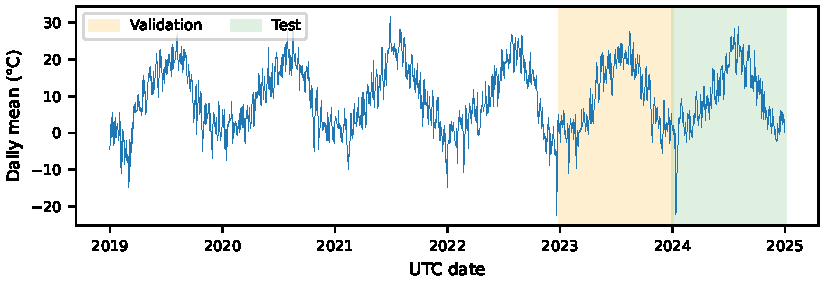
\includegraphics[width=\linewidth]{figures/data.pdf}
\captionof{figure}{Daily temperatures and the fixed evaluation partitions.
The strong annual cycle motivates known future calendar predictors.}
\end{center}

\newpage
\section{Methodology}
\subsection{Seasonal regression with ARMA/ARIMA errors}
Let $t$ be elapsed calendar days since January 1, 2019. For a fixed annual
period $P=365.25$, the model is
\begin{align}
y_t &= s_t+u_t,\\
s_t &= \beta_0+\sum_{k=1}^{K}\left[
a_k\sin\left(\frac{2\pi kt}{P}\right)+
b_k\cos\left(\frac{2\pi kt}{P}\right)\right].\label{eq:season}
\end{align}
The $k$th sine--cosine pair represents a harmonic with period $P/k$.
Increasing $K$ permits a more flexible seasonal profile while retaining a
low-dimensional parameterization. The fractional period approximates annual
seasonality rather than exact calendar anniversaries. A common time origin
preserves phase across data partitions and missing observations. The seasonal
coefficients are constant within each evaluation period.

The residual process satisfies
\begin{equation}
\phi(B)(1-B)^d u_t=\theta(B)\varepsilon_t,
\quad \varepsilon_t\sim\mathcal{N}(0,\sigma^2),
\end{equation}
where $B$ is the lag operator,
$\phi(B)=1-\sum_{j=1}^{p}\phi_jB^j$, and
$\theta(B)=1+\sum_{j=1}^{q}\theta_jB^j$.
When $d=0$, the specification reduces to ARMA$(p,q)$ errors. If diagnostic
evidence supports $d=1$, the regression intercept is omitted because
differencing eliminates its contribution. This formulation follows dynamic
harmonic regression \cite{hyndman2021}. The training diagnostics reported below
support $d=0$ for the combined models evaluated here.

Regression coefficients, ARMA parameters, and innovation variance are estimated
jointly by maximum likelihood using the SARIMAX state-space implementation
in \texttt{statsmodels} \cite{statsmodels}. An intercept is included in the
Fourier design matrix, with no additional SARIMAX trend. Parameter estimation
enforces stationarity and invertibility. Conditional on the information
available through origin $t$, the forecast decomposes as
\begin{equation}
\widehat y_{t+h\mid t}=\widehat s_{t+h}+\widehat u_{t+h\mid t}.
\end{equation}
The seasonal term is determined by the future date, whereas the residual
expectation is obtained recursively from the filtered state. Prediction
intervals are derived from the conditional state-space forecast distribution
for future observations, treating estimated parameters as fixed.

\subsection{Baseline models and component attribution}
\textbf{Persistence} uses $\widehat y_{t+h\mid t}=y_t$ at both horizons,
providing a reference based solely on the most recent observed temperature.
All evaluated origins have an observed value of $y_t$.

\textbf{Seasonal regression} retains Equation~\ref{eq:season} with independent
Gaussian errors, implemented as ARIMA$(0,0,0)$ errors. This baseline isolates
the predictive contribution of deterministic annual structure.

\textbf{Nonseasonal ARIMA} omits Fourier predictors and searches
$p,q\in\{0,1,2,3\}$ with $d\in\{0,1\}$. A constant is included for
$d=0$ and omitted for $d=1$; differenced candidates have no drift.
This family represents serial dependence without explicit annual regressors.

The \textbf{combined model} includes both Fourier predictors and residual
dynamics. Its candidate set contains ARMA$(0,0)$, nesting the independent-error
seasonal baseline. Consequently, validation can select a model without
residual dependence if that restriction improves predictive accuracy.

\subsection{Parameter interpretation}
The selected $K=3$ model refitted through 2023 has seasonal intercept
9.254\,$^\circ$C, $\widehat\phi_1=0.621$, $\widehat\theta_1=0.358$, and
$\widehat\sigma^2=5.623$\,$^\circ$C$^2$. For ARMA(1,1), residual mean forecasts
beyond the first step decay by successive powers of $\widehat\phi_1$.
This decay implies progressively smaller contributions from recent residual
information at longer horizons. Complete coefficient estimates are retained
with the reproducibility artifacts and remain fixed throughout testing.

\newpage
\section{Experimental design}
\subsection{Chronological validation and model selection}
Candidate parameters are estimated from 2019--2022. Validation proceeds through
2023 using daily forecast origins, with fixed parameters and sequential state
updates. The first origin is December 31, 2022. Eligibility requires the target
date to fall within 2023, yielding 365 one-day and 359 seven-day predictions.
The first seven-day target is January 7. Every model is evaluated on the
same origin--target pairs, ensuring comparability across specifications.

We search $K\in\{1,2,3\}$ and $p,q\in\{0,1,2,3\}$ for combined models.
Training ordinary seasonal-regression residuals are checked with augmented
Dickey--Fuller and KPSS tests. We consider $d=1$ for a harmonic count only if
ADF does not reject a unit root at 5\% and KPSS rejects level stationarity at
5\%. No harmonic count satisfies both conditions. This results in 48 combined
candidates, three independent-error seasonal candidates, and 32 nonseasonal
ARIMA candidates: 83 fits in total. All converge. These stationarity checks
are preliminary diagnostics; their residual input drops the single missing
training value and therefore closes one calendar gap. The likelihood fits and
forecast calendars preserve that gap.

One specification is selected within each model family by minimizing the
equal-weight mean of validation RMSE across the two horizons:
\begin{equation}
S(m)=\tfrac12\left(\operatorname{RMSE}_{1}(m)+
\operatorname{RMSE}_{7}(m)\right).
\end{equation}
Both components are expressed in Celsius. This criterion selects a common
specification across horizons and makes the weighting of short- and
longer-horizon accuracy explicit.

We record AIC, convergence warnings, parameters, and residual checks, but AIC
does not determine the selected family specifications. Nonconverged fits would
be excluded. The optimizer uses up to 300 iterations with a Powell-assisted
retry if needed, followed by another likelihood optimization.

\subsection{Held-out evaluation and information constraints}
Following model selection, each retained specification is refitted on
2019--2023. Orders are recorded before evaluating 2024, and all parameter
estimates remain fixed throughout the test period. At origin $t$, the model
uses only observations available through $t$ to generate predictions at
$t+1$ and $t+7$. The next observation is incorporated through a filtering
update only after these predictions have been recorded. Repeating this
operation produces daily rolling-origin forecasts without parameter refitting.

The first test origin is December 31, 2023. Target-date restrictions yield
366 one-day and 360 seven-day predictions. In particular, observations between
$t$ and $t+7$ cannot influence the forecast issued at $t$ for the seven-day
target. The information-availability assumption is that completed UTC-day
summaries are available at the origin. Actual publication delays are outside
the evaluation protocol.

\subsection{Evaluation criteria and protocol verification}
For errors $e_i=\widehat y_i-y_i$ over $n$ eligible targets, we report
$\operatorname{RMSE}=\sqrt{n^{-1}\sum_i e_i^2}$ and
$\operatorname{MAE}=n^{-1}\sum_i|e_i|$ separately by horizon.
For the combined model, coverage is $n^{-1}\sum_i\mathbf{1}\{L_i\leq y_i\leq U_i\}$
and mean width is $n^{-1}\sum_i(U_i-L_i)$ for nominal 95\% intervals.
Implementation checks verify horizon alignment and common target sets.
A perturbation check confirms that changing future observations leaves
previously issued forecasts unchanged.

\newpage
\section{Validation results and selected specifications}
Table~\ref{tab:validation} presents validation performance for the selected
specification in each family. Seasonal regression retains three Fourier pairs,
the nonseasonal baseline retains ARIMA$(3,0,3)$, and the combined model retains
three harmonic pairs with ARMA$(1,1)$ errors. The latter comprises seven
seasonal coefficients, two dependence parameters, and an innovation variance.
Selection therefore favors a lower-order residual process within the
specified search space.

\begin{center}
\captionof{table}{2023 validation metrics. Each model is fitted on 2019--2022.
One-day metrics use 365 targets and seven-day metrics use 359.}
\label{tab:validation}
\begin{tabular}{lrrrr}
\toprule
& \multicolumn{2}{c}{One day} & \multicolumn{2}{c}{Seven days}\\
Model & RMSE & MAE & RMSE & MAE\\
\midrule
Persistence & 2.441 & 1.881 & 5.248 & 4.039\\
Seasonal ($K=3$) & 3.661 & 2.896 & \textbf{3.672} & \textbf{2.903}\\
ARIMA$(3,0,3)$ & 2.259 & 1.763 & 4.457 & 3.429\\
Combined ($K=3$, ARMA$(1,1)$) & \textbf{2.169} & \textbf{1.703} & 3.677 & 2.906\\
\bottomrule
\end{tabular}
\end{center}

The one-day results indicate that recent observations contain information
beyond the deterministic calendar mean. Persistence outperforms seasonal
regression, and nonseasonal ARIMA improves further. The combined model attains
the lowest one-day RMSE, 2.169\,$^\circ$C, suggesting an additional contribution
from explicit seasonal predictors. At seven days, seasonal regression yields
a marginally lower RMSE than the combined model, 3.672 versus
3.677\,$^\circ$C. Both substantially outperform persistence and nonseasonal
ARIMA at this horizon.

These comparisons indicate a horizon-dependent contribution of residual
dynamics. Their incremental predictive value is evident at one day but
negligible at seven days in validation. The cross-horizon selection criterion
identifies a common combined specification without implying improvement
over the seasonal baseline at every horizon.

Training ADF p-values for the three seasonal residual series range from about
$1.2\times10^{-14}$ to $4.5\times10^{-12}$. KPSS reports 0.1 for each;
this is a lookup-table bound, not an exact p-value. These checks support the
decision to omit differencing in the combined-model search.

\begin{center}
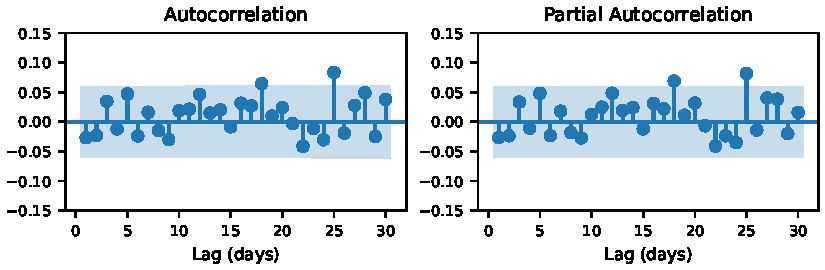
\includegraphics[width=\linewidth]{figures/acf.pdf}
\captionof{figure}{ACF and PACF of the selected combined model's standardized
training innovations. The longest continuous observed segment is used after
a 30-day burn-in. Shading is the plotting routine's nominal pointwise band.}
\label{fig:acf}
\end{center}

For this continuous segment, Ljung--Box tests yield p-values of 0.517 and
0.169 at lags 14 and 30, respectively, with degrees of freedom adjusted by
$p+q$. Figure~\ref{fig:acf} shows limited remaining autocorrelation.
The plotted bands are pointwise rather than simultaneous bounds across
lags. Failure to reject residual autocorrelation at these lags provides
diagnostic support for the conditional mean specification, but does not
establish normality or homoscedasticity.

\newpage
\section{Held-out point forecast performance}
Table~\ref{tab:test} reports held-out performance after refitting the selected
models on 2019--2023. The combined model attains the lowest observed RMSE
and MAE at both horizons. Its one-day RMSE is 2.405\,$^\circ$C, compared
with 2.578 for persistence, 4.003 for seasonal regression, and 2.486 for
nonseasonal ARIMA. The one-day ordering is consistent with validation and
supports the joint representation of annual structure and residual dependence.

\begin{center}
\captionof{table}{2024 held-out point forecast metrics in Celsius. The common
sample has 366 one-day and 360 seven-day targets. Bold indicates the minimum
within each column; it does not indicate a significance test.}
\label{tab:test}
\begin{tabular}{lrrrr}
\toprule
& \multicolumn{2}{c}{One day} & \multicolumn{2}{c}{Seven days}\\
Model & RMSE & MAE & RMSE & MAE\\
\midrule
Persistence & 2.578 & 1.978 & 5.556 & 4.371\\
Seasonal & 4.003 & 2.995 & 4.034 & 3.028\\
Nonseasonal ARIMA & 2.486 & 1.932 & 4.903 & 3.787\\
Combined & \textbf{2.405} & \textbf{1.815} & \textbf{4.019} & \textbf{3.022}\\
\bottomrule
\end{tabular}
\end{center}

Relative to persistence, the combined specification reduces test RMSE by
approximately 6.7\% at one day and 27.7\% at seven days. Reductions relative
to nonseasonal ARIMA are approximately 3.2\% and 18.0\%, respectively.
However, the seven-day improvement over persistence principally reflects the
contribution of annual structure: seasonal regression alone achieves nearly
the same accuracy as the combined model.

At seven days, the combined and seasonal models have RMSEs of 4.019\,$^\circ$C
and 4.034\,$^\circ$C. The difference using unrounded scores is approximately
0.015\,$^\circ$C, or 0.37\% of the seasonal baseline's RMSE. The corresponding
MAE difference is approximately 0.005\,$^\circ$C. This small advantage,
together with the reversed ordering in validation, limits the evidence for a
material seven-day benefit from residual dependence modeling.

\begin{center}
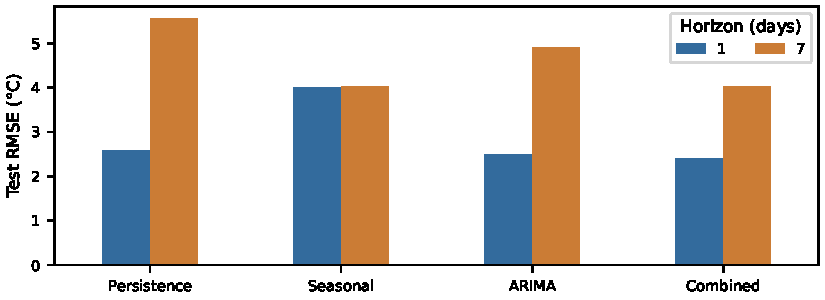
\includegraphics[width=\linewidth]{figures/accuracy.pdf}
\captionof{figure}{Test RMSE by model and horizon. Explicit annual seasonality
is particularly valuable for seven-day forecasts; residual dynamics substantially
improve on calendar-only regression at one day.}
\end{center}

All comparisons use identical target dates, eliminating target-subset
composition as an explanation for the observed differences. Nevertheless,
these estimates describe one station and one test year. No statistical
significance tests are reported, and overlapping seven-day errors are not
assumed independent. The results therefore support conditional conclusions
about this evaluation setting rather than general model dominance.

\newpage
\section{Prediction intervals and residual diagnostics}
\begin{center}
\captionof{table}{Combined-model nominal 95\% prediction intervals in the 2024
test. Width is measured in Celsius. Coverage is empirical over observed targets.}
\begin{tabular}{lrrr}
\toprule
Horizon & Targets & Coverage & Mean width\\
\midrule
One day & 366 & 93.7\% & 9.295\\
Seven days & 360 & 95.6\% & 14.856\\
\bottomrule
\end{tabular}
\end{center}

Mean interval width increases with horizon, from 9.295\,$^\circ$C at one day
to 14.856\,$^\circ$C at seven days, reflecting increased forecast uncertainty.
Seven-day aggregate coverage is close to the nominal level, whereas one-day
coverage is 93.7\%. Point forecast improvement consequently does not imply
nominal empirical coverage. Joint consideration of coverage and width is
necessary because wider intervals may improve coverage at the expense of
precision.

\begin{center}
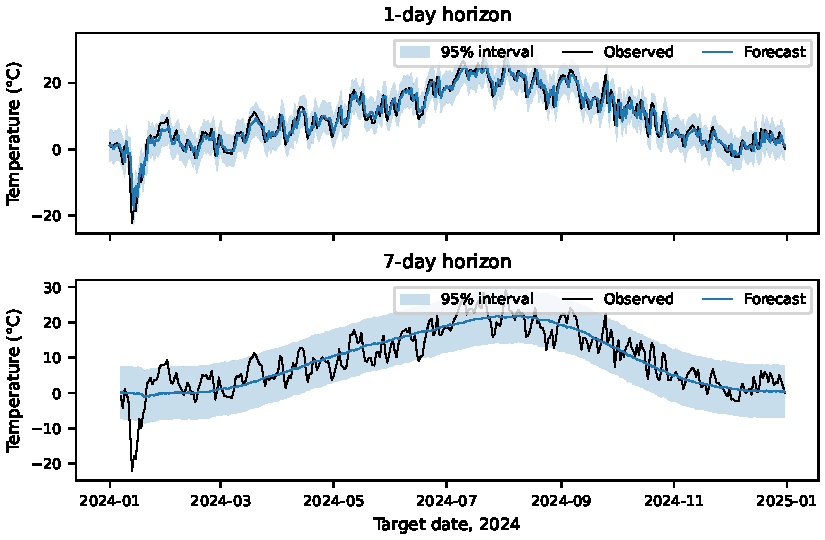
\includegraphics[width=\linewidth]{figures/forecasts.pdf}
\captionof{figure}{Rolling test predictions and conditional 95\% intervals.
Each plotted forecast is issued at its own origin; these curves are not a
single forecast issued at the start of 2024. The seven-day forecast closely
tracks the seasonal mean and misses the sharp January cold departure.}
\end{center}

After refitting, the combined model yields Ljung--Box p-values of 0.459 and
0.158 at lags 14 and 30. Diagnostics are computed on the longest uninterrupted
observed innovation segment, comprising 1,065 days after accounting for burn-in
and the missing observation. In contrast, the Jarque--Bera test rejects
normality ($p\approx5.1\times10^{-13}$), and the ARCH LM test with 14 lags
returns $p=0.025$, indicating evidence of conditional heteroscedasticity.
An adequate representation of serial mean dependence therefore does not
ensure adequacy of the innovation distribution.

The Gaussian intervals condition on estimated coefficients and exclude
parameter uncertainty. Their reported performance evaluates the original
specification without recalibration against held-out outcomes. Alternative
distributional assumptions or variance dynamics require a separate validation
exercise before a further test evaluation.

\newpage
\section{Discussion and limitations}
\subsection{Seasonal heterogeneity in forecast performance}
We group test targets into December--February (DJF), March--May (MAM),
June--August (JJA), and September--November (SON). DJF combines January and
February 2024 with December 2024; it is a seasonal category, not a single
contiguous winter episode. There are 91, 92, 92, and 91 one-day targets in
these groups. The seven-day winter group has 85 targets because the first
six January dates are not seven-day targets under our origin rule.

\begin{center}
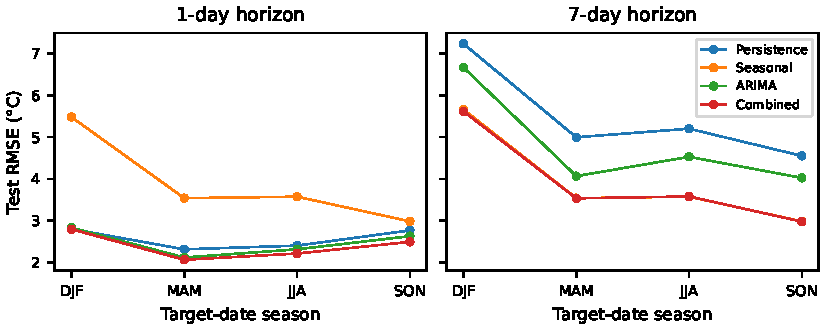
\includegraphics[width=\linewidth]{figures/seasons.pdf}
\captionof{figure}{Target-season RMSE. Winter is the most difficult season
at both horizons. Lines connect seasonal categories for readability and do not
represent an interpolated time series or confidence intervals.}
\end{center}

The combined model exhibits its largest errors in winter, with RMSEs of
2.794\,$^\circ$C and 5.616\,$^\circ$C at one and seven days, respectively.
Seven-day RMSE declines to 3.534 in spring, 3.579 in summer, and 2.977 in
autumn. Aggregate accuracy thus conceals substantial seasonal heterogeneity.
The January cold departure visible in the forecast trajectories contributes
to winter error, although this descriptive comparison does not identify the
causes of individual forecast failures.

Winter interval coverage is 91.2\% at one day and 87.1\% at seven days.
Seven-day coverage in spring, summer, and autumn is 98.9\%, 96.7\%, and
98.9\%, respectively. Near-nominal annual coverage therefore combines winter
undercoverage with relatively high coverage in other seasons. This
heterogeneity limits the interpretation of aggregate calibration for
weather-sensitive decisions, particularly during cold periods.

\subsection{Scope and external validity}
The predictor set contains only historical station observations and calendar
terms. Consequently, the model has no direct access to atmospheric information
that could anticipate changing weather regimes. The study establishes a
transparent statistical benchmark, while leaving comparison with operational
weather prediction systems outside its scope.

The six-year record provides four years for initial estimation and one year
each for validation and testing. Geographic and temporal generalization remain
limited by the single-station, single-test-year design. Coverage checks do not
constitute independent verification of every source measurement. In addition,
the fixed seasonal curve excludes secular trends and year-specific changes
in seasonal shape.

The evaluation distinguishes sequential state adaptation from parameter
re-estimation. It does not quantify the potential benefit of periodic
refitting. The assumption of immediate availability of completed daily
summaries further limits operational interpretation. Deployment would require
alignment between forecast origins and actual data-release times, followed
by prospective validation under those information constraints.

\newpage
\section{Reproducibility and conclusions}
\subsection{Computational reproducibility}
The implementation comprises Python scripts for station auditing,
preprocessing, model selection, rolling-origin evaluation, and result
generation, together with an executed demonstration notebook. Original inputs
are cached locally. Download manifests and SHA-256 checksums identify the
source files, while reproduction hashes link the processed series, analysis
code, evaluation protocol, and metric tables. Candidate forecasts and fitted
parameter records permit independent inspection of the reported comparisons.
The recorded environment uses Python 3.13.12, NumPy 2.4.3, pandas 3.0.1,
statsmodels 0.14.6, and Matplotlib 3.10.8.

The notebook reconstructs a forecast from fixed coefficients using observations
available only through a specified origin, and verifies its predictions and
interval endpoints against the saved rolling evaluation. Additional protocol
checks cover Fourier phase across leap days, exact horizon alignment,
parameter preservation, and invariance of earlier forecasts to perturbations
of future observations. All ten notebook code cells execute successfully.
These checks establish implementation consistency rather than external
predictive validity. Source code and artifacts accompany the study at
\url{https://github.com/lamanmirzayeva/Weather-Forecasting}.

\subsection{Conclusions and future research}
The results provide evidence that annual Fourier regression and ARMA residual
dynamics offer complementary information for one-day temperature forecasting
at the studied station. The combined model achieves the lowest one-day RMSE
in both chronological validation and held-out testing. At seven days, the
incremental test improvement over seasonal regression is small and the
validation ordering differs, indicating that annual structure accounts for
most of the observed predictive benefit at that horizon.

Uncertainty evaluation yields a more qualified conclusion. Aggregate seven-day
coverage is near nominal, but winter undercoverage, nonnormal innovations,
and evidence of changing variance reveal limitations of the Gaussian
constant-variance specification. Future research should assess alternative
innovation distributions and variance models, additional stations, and
prospective test years. Such extensions require renewed chronological
validation rather than selection against the completed 2024 test.

\begin{thebibliography}{9}
\raggedright
\bibitem{hyndman2021} R. J. Hyndman and G. Athanasopoulos. \emph{Forecasting: Principles and
Practice}, 3rd ed. OTexts, 2021. Chapter 10, Dynamic regression models,
including dynamic harmonic regression.
\url{https://otexts.com/fpp3/dynamic-regression.html}.
\bibitem{hyndman2008} R. J. Hyndman and Y. Khandakar. Automatic time series forecasting:
the forecast package for R. \emph{Journal of Statistical Software}, 27(3):1--22,
2008. \url{https://doi.org/10.18637/jss.v027.i03}.
\bibitem{taylor2018} S. J. Taylor and B. Letham. Forecasting at scale.
\emph{The American Statistician}, 72(1):37--45, 2018.
\url{https://doi.org/10.1080/00031305.2017.1380080}.
\bibitem{noaa} NOAA National Centers for Environmental Information. \emph{Global Surface
Summary of the Day (GSOD)}. Dataset and field documentation.
\url{https://www.ncei.noaa.gov/data/global-summary-of-the-day/access/};
\url{https://www.ncei.noaa.gov/data/global-summary-of-the-day/doc/readme.txt}.
\bibitem{statsmodels} The statsmodels Developers. \emph{SARIMAX: State-Space Time-Series
Modeling}, version 0.14.6. Model and forecast-state update documentation.
\url{https://www.statsmodels.org/v0.14.6/generated/statsmodels.tsa.statespace.sarimax.SARIMAX.html}.
\end{thebibliography}
\end{document}
